\documentclass{article}
\usepackage[utf8]{inputenc}
\usepackage{amsmath}
\usepackage{graphicx}
\usepackage{tabularx}
\usepackage{xcolor}
\usepackage{tabularray}
\usepackage{float}
\usepackage{bm}
\usepackage[colorlinks]{hyperref}
\usepackage[normalem]{ulem}
\usepackage[affil-it]{authblk}
\setlength{\parindent}{0pt}
\usepackage{caption}
\captionsetup[table]{position=bottom} 
%\usepackage{draftwatermark}
%\SetWatermarkText{Draft}
%\SetWatermarkScale{4}
%\SetWatermarkColor[gray]{0.97}

\usepackage{titlesec}

\setcounter{secnumdepth}{4}

\titleformat{\paragraph}
{\normalfont\normalsize\bfseries}{\theparagraph}{1em}{}
\titlespacing*{\paragraph}
{0pt}{3.25ex plus 1ex minus .2ex}{1.5ex plus .2ex}

\title{Analysis of UN Actors in the PA-X Agreement-Actor Signatories Dataset}
\author{Roy Gardner}

\begin{document}

\newcolumntype{R}{>{\raggedleft\arraybackslash}X}

\maketitle

\tableofcontents
\newpage

\section{Introduction}

\subsection{List of UN Actors}

\begin{table}[H]
\begin{center}
\small
\begin{tabularx}{\textwidth}{|X|l|}
    \hline
    \textbf{Name} & \textbf{Identifier} \\
    \hline
    \hline
        Group of Friends UNSG & COA\_51 \\
	\hline
	Office of the United Nations High Commissioner for Human Rights & IGO\_640 \\
	\hline
	UN General Assembly & IGO\_315 \\
	\hline
	UN Office on Drugs and Crimes & IGO\_672 \\
	\hline
	UN Secretary General & IGO\_386 \\
	\hline
	UN Security Council & IGO\_8 \\
	\hline
	UNAMID & IGO\_950 \\
	\hline
	UNAMSIL & IGO\_652 \\
	\hline
	UNCRO & IGO\_795 \\
	\hline
	UNISFA & IGO\_616 \\
	\hline
	UNMIBH & IGO\_405 \\
	\hline
	UNMIS & IGO\_854 \\
	\hline
	UNMISS & IGO\_831 \\
	\hline
	UNMOT & IGO\_454 \\
	\hline
	UNOMB & IGO\_274 \\
	\hline
	UNOMIG & IGO\_480 \\
	\hline
	UNPOS & IGO\_536 \\
	\hline
	UNPROFOR & IGO\_355 \\
	\hline
	UNSMIL & IGO\_750 \\
	\hline
	United Nations (General) & IGO\_49 \\
	\hline
	United Nations Children's Fund & IGO\_459 \\
	\hline
	United Nations Development Programme & IGO\_64 \\
	\hline
	United Nations Educational, Scientific and Cultural Organization & IGO\_678 \\
	\hline
	United Nations Human Rights Council & IGO\_440 \\
	\hline
	United Nations Population Fund & IGO\_674 \\
	\hline
	United Nations Secretariat & IGO\_391 \\
	\hline
\end{tabularx}
\end{center}
\normalsize
\caption{Names and identifiers of 26 UN actors obtained from the PA-X agreement-actor signatories dataset. }
\end{table}

\subsection{Numerical data}

\begin{table}[H]
\begin{center}
\small
\begin{tabularx}{\textwidth}{|X|r|}
    \hline
    \textbf{Variable} & \textbf{Value} \\
    \hline
    \hline
     Number of agreements in dataset & 1642 \\
     \hline
     Number of actors in dataset & 1092 \\
     \hline
     Number of UN actors in dataset (see Table 1 above) & 26 \\
     \hline
     Number of agreements to which one or more UN actors are signatories & 371 \\
     \hline
     Number of non-UN actors that are co-signatories with UN actors  & 510  \\
     \hline
\end{tabularx}
\end{center}
\normalsize
\caption{Basic numerical data.}
\end{table}

\begin{table}[H]
\begin{center}
\small
\begin{tabularx}{\textwidth}{|X|r|}
    \hline
    \textbf{Variable} & \textbf{Value (\%))} \\
    \hline
    \hline
     UN actors as a percentage of all actors  & 2.4  \\
     \hline
     Agreements signed by UN actors as a percentage of all agreements  & 22.6  \\
     \hline
     UN actor co-signatories as a percentage of all actors & 46.7  \\
     \hline
\end{tabularx}
\end{center}
\normalsize
\caption{Derived numerical data.}
\end{table}

\subsection{Number of agreements signed by UN actors}


\begin{figure}[H]
\begin{center}
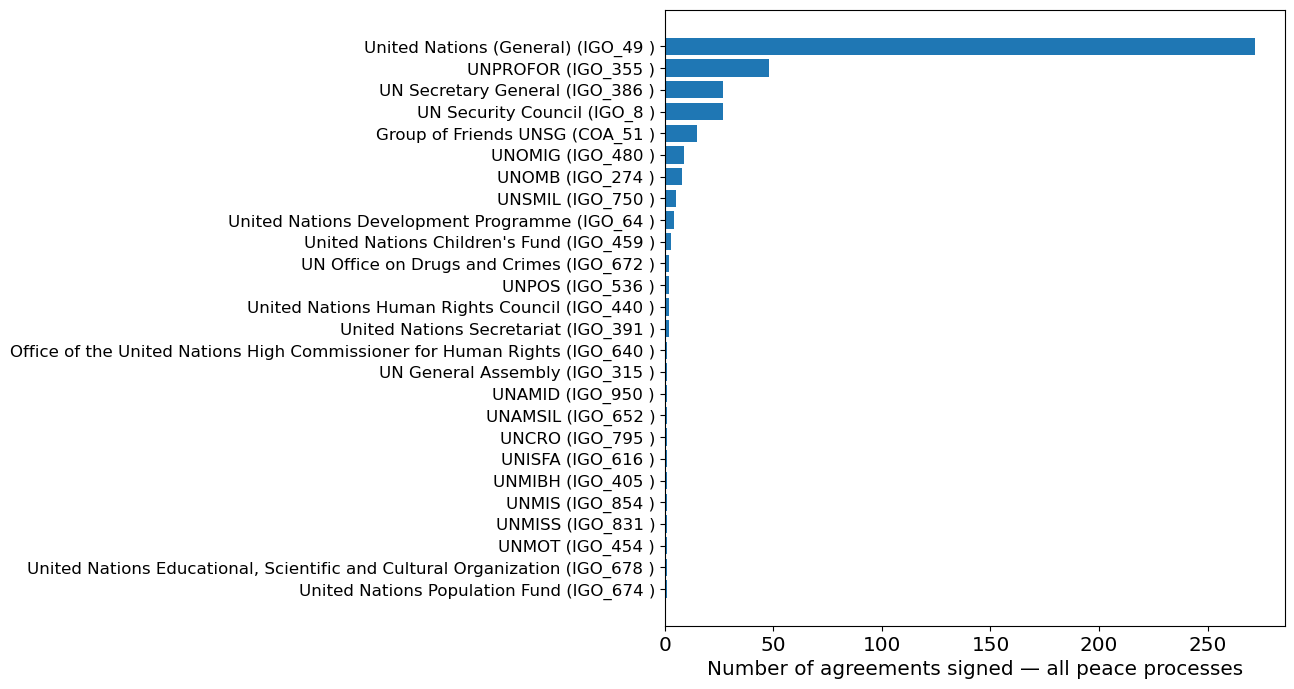
\includegraphics[scale=0.36]{./assets/figure_1.png}
\caption{Plot showing number of agreements signed by the 26 UN actors in the analysis. See Table 3 below for exact values.}
\end{center}
\end{figure}

\begin{table}[H]
\begin{center}
\small
\begin{tabularx}{\textwidth}{|X|r|}
    \hline
    \textbf{UN actor} & \textbf{Number of agreements signed} \\
    \hline
    \hline
United Nations (General) & 272 \\
\hline
UNPROFOR & 48 \\
\hline
UN Secretary General & 27 \\
\hline
UN Security Council & 27 \\
\hline
Group of Friends UNSG & 15 \\
\hline
UNOMIG & 9 \\
\hline
UNOMB & 8 \\
\hline
UNSMIL & 5 \\
\hline
United Nations Development Programme & 4 \\
\hline
United Nations Children's Fund & 3 \\
\hline
UN Office on Drugs and Crimes & 2 \\
\hline
UNPOS & 2 \\
\hline
United Nations Human Rights Council & 2 \\
\hline
United Nations Secretariat & 2 \\
\hline
Office of the United Nations High Commissioner for Human Rights & 1 \\
\hline
UN General Assembly & 1 \\
\hline
UNAMID & 1 \\
\hline
UNAMSIL & 1 \\
\hline
UNCRO & 1 \\
\hline
UNISFA & 1 \\
\hline
UNMIBH & 1 \\
\hline
UNMIS & 1 \\
\hline
UNMISS & 1 \\
\hline
UNMOT & 1 \\
\hline
United Nations Educational, Scientific and Cultural Organization & 1 \\
\hline
United Nations Population Fund & 1 \\
\hline
\end{tabularx}
\end{center}
\normalsize
\caption{Number of agreements signed by UN actors in descending order. See Figure 1 above.}
\end{table}


\end{document}
















